\documentclass{beamer}

\def\draft{draft}
\def\final{final}
\def\status{draft}
% !TeX root = ../thesis_presentation.tex
\usepackage[utf8]{inputenc}
\usepackage[T1]{fontenc}
\usepackage{lmodern}
\usepackage{times}
\usepackage[american]{babel}
\usepackage{tikz}
\usepackage{listings}
\usepackage{subcaption}
\usepackage{bm}
\usepackage{booktabs}
\usepackage{amsfonts}
\usepackage{amsmath}
\usepackage{amssymb}
\usepackage{amsthm}
\usepackage{marvosym}
\let\marvosymLightning\Lightning


%	Settings
%======================================================================
%%Tikz
\usetikzlibrary{shapes,arrows,calc,positioning,fit}

%% THEME: UOS-red or UOS-yellow
\usetheme{UOS}
% \usetheme[uosyellow]{UOS}

%% where to find the graphics
\graphicspath{{img/}}

%% Command setup
\newcommand{\source}[1]{\caption*{\textcolor{uos-grey-full}{Source: {#1}}} }
\newcommand{\RM}[1]{\MakeUppercase{\romannumeral{} #1{}}}
\newcommand{\code}[1]{\texttt{#1}}
\newcommand{\bull}[0]{\textbullet{}}
\newcommand{\tabitem}{{\color{uos-red-full}$\blacksquare$}}

% ---------------------------------------------------------------------
%% insert outline at begin of every section
\AtBeginSection[]{
  \frame{
    \frametitle{\iflanguage{ngerman}{Gliederung}{Outline}}
    \tableofcontents[current, currentsubsection]
  }
}

%% format: \title[short title]{long title}
%%   - short title will be used in foot line
%%   - long title will be used on title page
\title[Development with DevContainers]{Analysis of Adopting DevOps Tools for a Homogeneous Production and Development Environment}

% Color
\definecolor{codebg}{HTML}{EEEEEE}
\definecolor{dkgreen}{rgb}{0,0.6,0}
\definecolor{gray}{rgb}{0.5,0.5,0.5}
\definecolor{mauve}{rgb}{0.58,0,0.82}
\definecolor{LightCyan}{rgb}{0.88,1,1}


% Listings style file

\lstdefinelanguage{docker}{
  keywords={FROM, RUN, COPY, ADD, ENTRYPOINT, CMD,  ENV, ARG, WORKDIR, EXPOSE, LABEL, USER, VOLUME, STOPSIGNAL, ONBUILD, MAINTAINER},
  keywordstyle=\color{orange}\bfseries,
  identifierstyle=\color{black},
  % basicstyle=\small,
  sensitive=false,
  comment=[l]{\#},
  commentstyle=\color{blue}\ttfamily\emph,
  stringstyle=\color{dkgreen}\ttfamily\textbf,
  morestring=[b]',
  morestring=[b]"
}

\lstdefinelanguage{docker-compose}{
  keywords={image, environment, ports, container_name, ports, volumes, links},
  keywordstyle=\color{blue}\bfseries,
  identifierstyle=\color{black},
  sensitive=false,
  comment=[l]{\#},
  commentstyle=\color{purple}\ttfamily,
  stringstyle=\color{red}\ttfamily,
  morestring=[b]',
  morestring=[b]"
}
\lstdefinelanguage{docker-compose-2}{
  keywords={version, volumes, services, networks, image},
  keywordstyle=\color{blue}\bfseries,
  keywords=[2]{environment, ports, container_name, ports, links, build, expose, env_file, restart, depends_on}
  keywordstyle=[2]\color{olive}\bfseries,
  identifierstyle=\color{black},
  sensitive=false,
  comment=[l]{\#},
  commentstyle=\color{purple}\ttfamily,
  stringstyle=\color{red}\ttfamily,
  morestring=[b]',
  morestring=[b]"
}

\lstset{basicstyle=\ttfamily,
  inputencoding=utf8,
  extendedchars=true
  basicstyle=\footnotesize,       % the size of the fonts that are used for the code
  numbers=left,                   % where to put the line-numbers
  numberstyle=\tiny\color{gray},  % the style that is used for the line-numbers
  stepnumber=1,                   % the step between two line-numbers. If 1 = all lines numberd
  numbersep=5pt,                  % how far the line-numbers are from the code
  backgroundcolor=\color{white},  % choose the background color. You must add \usepackage{color}
  showspaces=false,               % show spaces adding particular underscores
  showstringspaces=false,         % underline spaces within strings
  showtabs=false,                 % show tabs within strings adding particular underscores
  frame=single,                   % adds a frame around the code
  rulecolor=\color{black},        % if not set, the frame-color may be changed on line-breaks
  tabsize=4,                      % sets default tabsize to 2 spaces
  captionpos=b,                   % sets the caption-position to bottom
  breaklines=true,                % sets automatic line breaking
  breakatwhitespace=false,        % sets if automatic breaks should only happen at whitespace
  title=\lstname,                 % show the filename of files included with \lstinputlisting;
  keywordstyle=\color{blue},      % keyword style
  commentstyle=\color{dkgreen},   % comment style
  stringstyle=\color{mauve}       % string literal style
}


%======================================================================
% * * * * * * *   T E X T    S T A R T S    H E R E   * * * * * * * * *
%======================================================================
\begin{document}

\begin{frame}[plain]
  \titlepage{}
\end{frame}

\begin{frame}[allowframebreaks]{\iflanguage{ngerman}{Inhaltsverzeichnis}{Table of Contents}}
  \tableofcontents
\end{frame}

%%%%%%%%%%%%%%%%%%%%%%%%%%%%%%%%%%%%%%%%%%%%%%%%%%%%%%%%%%%%%%%%%%%%%%%%%%%%%%%%
% NOTES:
%%%%%%%%%%%%%%%%%%%%%%%%%%%%%%%%%%%%%%%%%%%%%%%%%%%%%%%%%%%%%%%%%%%%%%%%%%%%%%%%
\section{Motivation \& Goal}
\begin{frame}{Goal of the Thesis}
  \begin{itemize}
    \large
    \setlength\itemsep{1em}
    \setlength{\parskip}{12pt}
    \item Possibilities to increase efficiency in programming
          \begin{itemize}
            \large
            \setlength\itemsep{1em}
            \item Investigate possible points of improvement
            \item Develop an abstract solution concept
            \item Apply the concept to a prototype
            \item Evaluate and compare the concept to alternative solutions
          \end{itemize}
  \end{itemize}
  \vfill
\end{frame}


%%%%%%%%%%%%%%%%%%%%%%%%%%%%%%%%%%%%%%%%%%%%%%%%%%%%%%%%%%%%%%%%%%%%%%%%%%%%%%%%
% NOTES:
% Studie von 2019 by ActiveState (Firma die sich auf coaching und Optimierung von Softwareprozessen spezialisiert)
% Habe mir dabei angesehen wie viele Stunden Entwickler nicht aktive coden
% Abseits von Software design und meeting Zeit sind dies die Tätigkeiten die am
% meisten Zeit in Anspruch nehmen.
% Neben Software Design und Meetings gehört auch Bug fixing dazu, dies hat aber
% Überschneidungen mit coding als auch mit Problemen in Konfigurationen und Dependencies
%%%%%%%%%%%%%%%%%%%%%%%%%%%%%%%%%%%%%%%%%%%%%%%%%%%%%%%%%%%%%%%%%%%%%%%%%%%%%%%%
\section{Restriction in Development Environments}
\begin{frame}{}
  \begin{center}
    \large{\color{uos-red-full} Potential Bottlenecks in the development workflow}
    \normalsize
    \vspace{0.5cm}
    \begin{columns}[totalwidth=\textwidth]
      \begin{column}{0.4\textwidth}
        \begin{itemize}
          \item Setup Configuration
          \item Testing
        \end{itemize}
      \end{column}
      \begin{column}{0.4\textwidth}
        \begin{itemize}
          \item Configuration
          \item Dependencies
        \end{itemize}
      \end{column}
    \end{columns}
  \end{center}

  \ifx\status\final{}
    \pause{}
  \fi

  \begin{figure}
    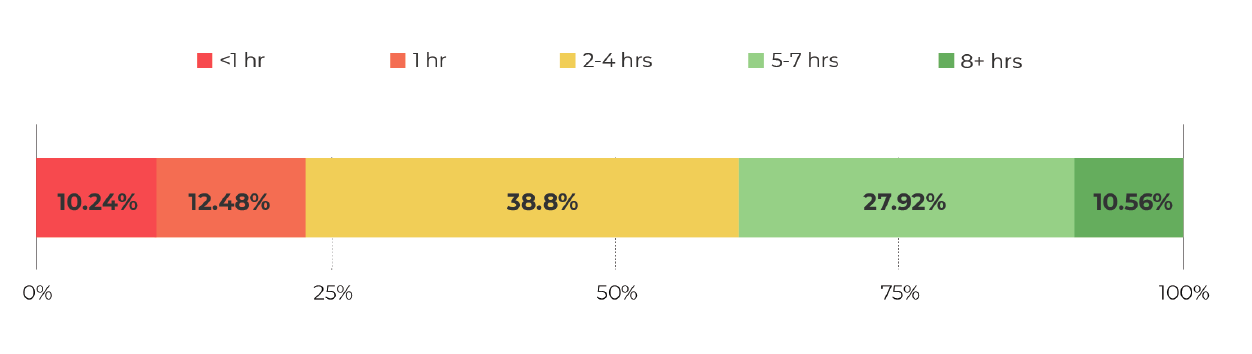
\includegraphics[width=0.8\textwidth]{coding_timepng.png}
    \caption{\footnotesize Hours spent programming \\\textcolor{uos-grey-full}{Source: {\cite{setuppain}}}}
  \end{figure}
\end{frame}

%%%%%%%%%%%%%%%%%%%%%%%%%%%%%%%%%%%%%%%%%%%%%%%%%%%%%%%%%%%%%%%%%%%%%%%%%%%%%%%%
% NOTES:
% Die Studie zeigt das die meisten Entwickler 1-4 mal im Jahr ihr System
% wechseln oder erneuern. Einige sogar deutlich öfter

% Dazu kommen neue Entwickler.
% Dies dauert bei den meisten 2-4 Stunden und bei 1/5 sogar zwischen 4 und 18 Stunden
% Für den GitHub.com Dienst haben die Entwickler ein scripts-to-rule-them-all geschrieben
% Dies dauerte allein 45 min für DB updates, oder dem installieren neuer dependencies beim wechseln von branches.
% Initiale Aufgaben wie E-Mail, VPN, Login für Git Lab/Hub, Jira etc. werden dabei nicht berücksichtigt
%%%%%%%%%%%%%%%%%%%%%%%%%%%%%%%%%%%%%%%%%%%%%%%%%%%%%%%%%%%%%%%%%%%%%%%%%%%%%%%%
\begin{frame}{}
  \vspace{-0.2cm}
  \begin{center}
    \Large Initial Setup
  \end{center}

  \begin{block}{}
    \begin{itemize}
      \small
      \setlength\itemsep{0em}
      \item 69\% of developers renew their setup between 1-4 times a year
      \item 18\% even 5-8 times a year
    \end{itemize}
  \end{block}

  \ifx\status\final{}
    \pause{}
  \fi


  \begin{block}{}
    \begin{itemize}
      \small
      \setlength\itemsep{0em}
      \item 44\% of developers need 2-4 hours to setup their environment
      \item 14\% spent 4-8 hours and 6\% even over 18 hours
    \end{itemize}
  \end{block}

  \ifx\status\final{}
    \pause{}
  \fi


  \begin{block}{}
    \begin{itemize}
      \small
      \setlength\itemsep{0em}
      \item Installing development tools, language frameworks and IDEs
      \item Logging into E-Mail, VPN, messenger and network-shares
    \end{itemize}
  \end{block}
\end{frame}

%%%%%%%%%%%%%%%%%%%%%%%%%%%%%%%%%%%%%%%%%%%%%%%%%%%%%%%%%%%%%%%%%%%%%%%%%%%%%%%%
% NOTES:
% Und am Ende hat man das:
% Es fehlt immer noch ein Programm, eine Bibliothek oder es wurde eine falsche
% Version installiert. Die bringt uns zum Configurations und Dependency management
%%%%%%%%%%%%%%%%%%%%%%%%%%%%%%%%%%%%%%%%%%%%%%%%%%%%%%%%%%%%%%%%%%%%%%%%%%%%%%%%
\begin{frame}{}
  \begin{center}
    \Large Intensive Setup
  \end{center}
  \begin{figure}
    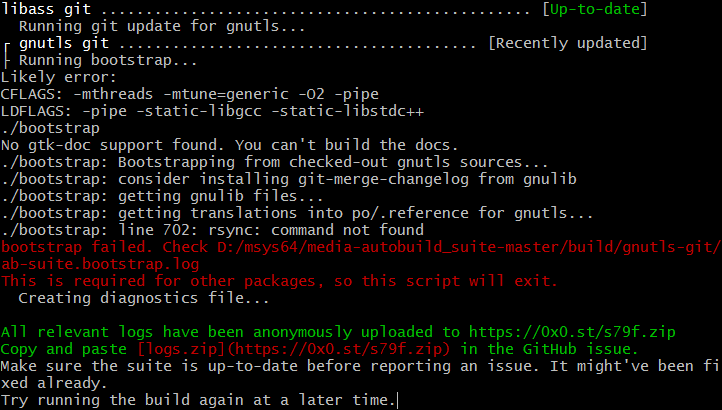
\includegraphics[width=0.8\textwidth]{img/terminal.png}
    \caption{Failed bootstrap script}
  \end{figure}
\end{frame}

%%%%%%%%%%%%%%%%%%%%%%%%%%%%%%%%%%%%%%%%%%%%%%%%%%%%%%%%%%%%%%%%%%%%%%%%%%%%%%%%
% NOTES:
% Das herstellen einer konsistenten und funktionierenden Entwicklungsumgebung
% über mehrere Entwickler (eventuell sogar verschiedene Betriebssysteme) ist eine
% enorme Herausforderung insbesondere in einer Microservice Architektur
% Man muss:
% Über Umgebungsvariablen werden in der regel Einstellungen wie HOST, PORT, USER und PW
% für Datenbanken und andere Einstellungen übergeben. Weiteres sind z.B. API Keys
% Die Komplexität nimmt exponential zu wenn man viele Anwendungen hat die auch noch untereinander Kommunizieren APP B -> zu APP A ...

% Oftmals gibt es dann auch noch unterschiede bei den Dependencies.
% Entwickler die an mehreren Projekten Arbeiten (häufig) müssen eventuelle
% NodJS 12 für ein Projekt und NodeJS 14 für ein anderes benutzen.
% Dazu kommen die zwischen Development und Production Umgebung.
% Production läuft oft Linux 75.3% aller Webserver (w3techs) & Development oft Windows 40% Linux 25% MacOs 25% StackOverflow 2021

% Einiges wird unter Windows auch nicht mehr unterstützt. Keine Entwicklung von Lagacy PHP unter Windows

%%%%%%%%%%%%%%%%%%%%%%%%%%%%%%%%%%%%%%%%%%%%%%%%%%%%%%%%%%%%%%%%%%%%%%%%%%%%%%%%
\begin{frame}{}
  \vspace{-.6cm}
  \begin{center}
    \Large Configuration \& Dependencies
  \end{center}

  \begin{block}{}
    \begin{itemize}
      \small
      \setlength\itemsep{0em}
      \item APP A needs a DB connection string with: host, user, password
      \item APP B listens on port 8080 and requests APP A on port 3000
    \end{itemize}
  \end{block}

  \ifx\status\final{}
    \pause{}
  \fi

  \begin{block}{}
    \begin{itemize}
      \small
      \setlength\itemsep{0em}
      \item Project A requires NodeJS V12 {\color{uos-red-full}\text{\marvosymLightning}} Project B requires NodeJS V14
      \item Development uses Python 3.9 {\color{uos-red-full}\text{\marvosymLightning}} Production uses Python 3.7
      \item Development uses PHP 7.3 {\color{uos-red-full}\text{\marvosymLightning}} Production uses legacy PHP \(\leq 7.0\)
    \end{itemize}
  \end{block}
\end{frame}

%%%%%%%%%%%%%%%%%%%%%%%%%%%%%%%%%%%%%%%%%%%%%%%%%%%%%%%%%%%%%%%%%%%%%%%%%%%%%%%%
% NOTES:
% Das sind nur die Runtime Dependencies - Dependencies zwischen Anwendungen können zur
% enormen Herausforderung werden. Alle einzelnen Anwendung müssen gestartet und dessen output überwacht werden

% Das sind alle Services die XXX bei Netflix liefen. Die wird NICHT alle lokal laufen lassen
% Aber allein ein Bruchteil davon auf dem lokalen auf dem PC zu installieren und zu starten kann schnell unübersichtlich und Fehleranfällig werden
% Wenn man ein Service Mesh hat dann ist Testing eine große Herausforderung, auch bei kleineren Diensten
% Alles andere wird zu aufwendig auf dem lokalen PC zu installieren.
% Zwar gibt es Mock Server, und API validations zum testen, diese garantieren jedoch nicht dass zwei Services wirklich erfolgreich kommunizieren können.
%%%%%%%%%%%%%%%%%%%%%%%%%%%%%%%%%%%%%%%%%%%%%%%%%%%%%%%%%%%%%%%%%%%%%%%%%%%%%%%%
% Deswegen können in einer MSA viele tests nur in der CI ausgeführt werden. Dort dauert es viel länger bis ein Fehler gefunden wird und das verlangsamt und verteuert den Entwicklungsprozess
\begin{frame}{}
  \begin{center}
    \Large Configuration \& Dependencies
  \end{center}
  \begin{figure}
    % 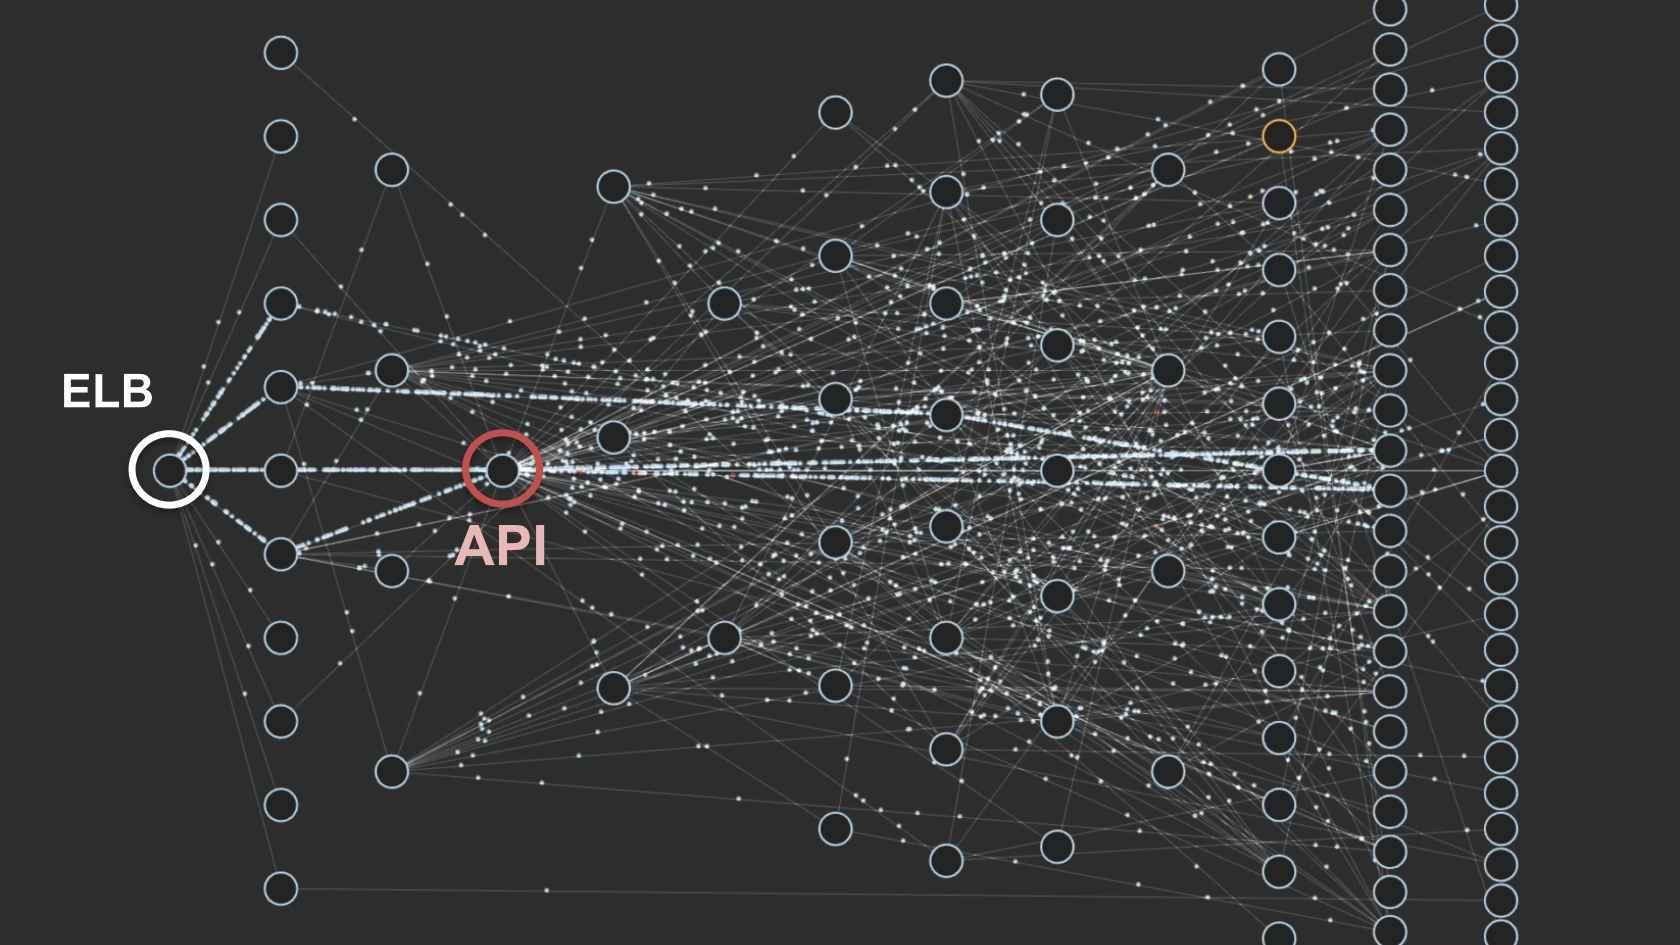
\includegraphics[width=0.8\textwidth]{img/netflix.jpg}
    % \caption{Netflix Microservice Graph}
    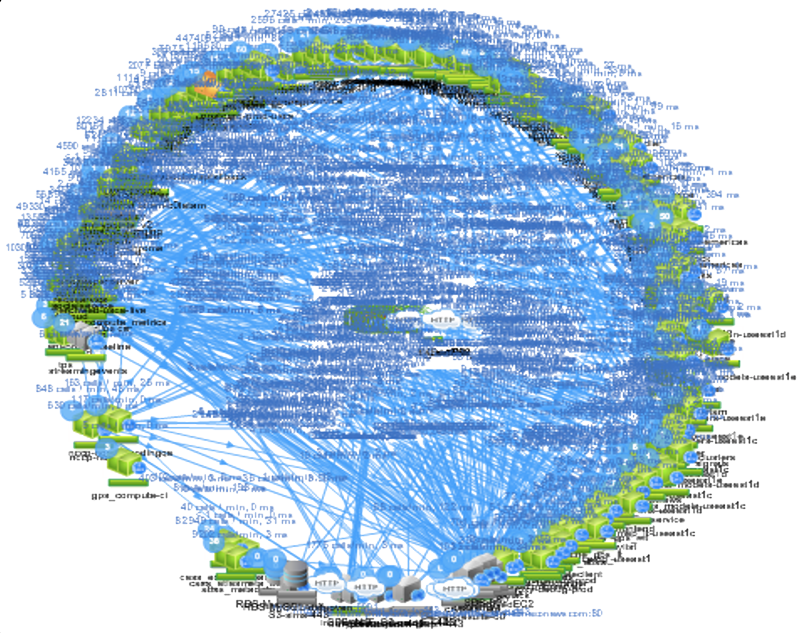
\includegraphics[width=0.6\textwidth]{img/netfix.png}
    \caption{\footnotesize Netflix's Microservice Death-Star \\\textcolor{uos-grey-full}{Source: {\cite{deathstar}}}}
  \end{figure}
\end{frame}


\section{Homogenization of Development Setups}
%%%%%%%%%%%%%%%%%%%%%%%%%%%%%%%%%%%%%%%%%%%%%%%%%%%%%%%%%%%%%%%%%%%%%%%%%%%%%%%%
% NOTES:
% PaaS
%%%%%%%%%%%%%%%%%%%%%%%%%%%%%%%%%%%%%%%%%%%%%%%%%%%%%%%%%%%%%%%%%%%%%%%%%%%%%%%%
\subsection{General Concept}
\begin{frame}{}
  \begin{center}
    \Large Apply solutions from the server world
  \end{center}
  \vspace{.8cm}

  \ifx\status\final{}
    \pause{}
  \fi

  \begin{itemize}
    \setlength\itemsep{1.2em}
    \large
    \item Abstract the underlying hardware and system
    \item Define and standardize the working environments
    \item Reduce manual effort and automate processes
    \item Allow app/test integration on the developer system
  \end{itemize}
\end{frame}

%%%%%%%%%%%%%%%%%%%%%%%%%%%%%%%%%%%%%%%%%%%%%%%%%%%%%%%%%%%%%%%%%%%%%%%%%%%%%%%%
% NOTES:
% PaaS
%%%%%%%%%%%%%%%%%%%%%%%%%%%%%%%%%%%%%%%%%%%%%%%%%%%%%%%%%%%%%%%%%%%%%%%%%%%%%%%%
\begin{frame}{}
  \begin{columns}[totalwidth=\textwidth]
    \begin{column}{0.5\textwidth}
      \begin{figure}
        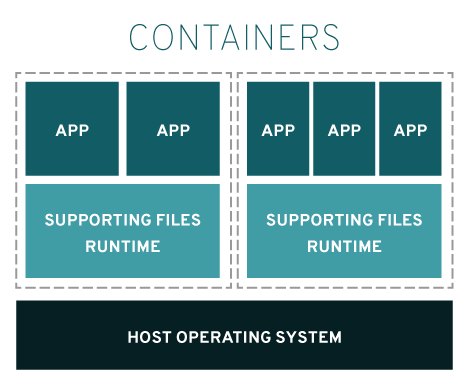
\includegraphics[width=1.1\textwidth]{img/docker-vm-redhat.png}
        \caption{\footnotesize Container-based virtualization - \textcolor{uos-grey-full}{Source: {\cite{redhat_pic}}}}
      \end{figure}
    \end{column}

    \ifx\status\final{}
      \pause{}
    \fi


    \begin{column}{0.4\textwidth}
      \begin{itemize}
        \setlength\itemsep{0.6em}
        \item Container-based virtualization
        \item Less resource needs than a VM; Only the process is isolated
        \item The app runtime is in a self-contained bundle
        \item Implemented with Docker
      \end{itemize}
    \end{column}
  \end{columns}
\end{frame}

%%%%%%%%%%%%%%%%%%%%%%%%%%%%%%%%%%%%%%%%%%%%%%%%%%%%%%%%%%%%%%%%%%%%%%%%%%%%%%%%
% NOTES:
% PaaS
%%%%%%%%%%%%%%%%%%%%%%%%%%%%%%%%%%%%%%%%%%%%%%%%%%%%%%%%%%%%%%%%%%%%%%%%%%%%%%%%
\begin{frame}{}
  \begin{block}{}
    \begin{itemize}
      \item Applying the IaC principle
      \item Docker provides a unified, independent platform
    \end{itemize}
  \end{block}

  \ifx\status\final{}
    \pause{}
  \fi


  \begin{block}{}
    \begin{itemize}
      \item Orchestrate and test multiple services
      \item Closer to the production environment
    \end{itemize}
  \end{block}

  \ifx\status\final{}
    \pause{}
  \fi


  \begin{block}{}
    \begin{itemize}
      \item Different projects are isolated from each other
      \item Wider choice of available software
    \end{itemize}
  \end{block}
\end{frame}

%%%%%%%%%%%%%%%%%%%%%%%%%%%%%%%%%%%%%%%%%%%%%%%%%%%%%%%%%%%%%%%%%%%%%%%%%%%%%%%%
% NOTES:
% PaaS
%%%%%%%%%%%%%%%%%%%%%%%%%%%%%%%%%%%%%%%%%%%%%%%%%%%%%%%%%%%%%%%%%%%%%%%%%%%%%%%%
\begin{frame}{}
  \vspace{-0.2cm}
  \begin{center}
    \large Architectural concept
  \end{center}
  \vspace{-0.4cm}
  \begin{figure}
    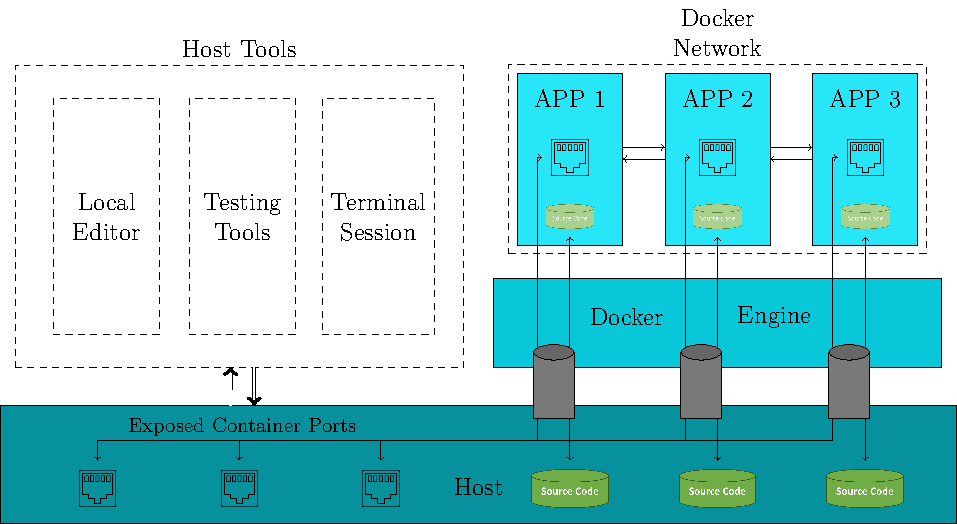
\includegraphics[width=\textwidth]{img/thesis_main-figure2.pdf}
    \caption{Development Architecture with DevContainers}
  \end{figure}
\end{frame}


%%%%%%%%%%%%%%%%%%%%%%%%%%%%%%%%%%%%%%%%%%%%%%%%%%%%%%%%%%%%%%%%%%%%%%%%%%%%%%%%
% NOTES:
% PaaS
%%%%%%%%%%%%%%%%%%%%%%%%%%%%%%%%%%%%%%%%%%%%%%%%%%%%%%%%%%%%%%%%%%%%%%%%%%%%%%%%
\begin{frame}{}
  \vspace{-.5cm}
  \begin{center}
    \begin{figure}
      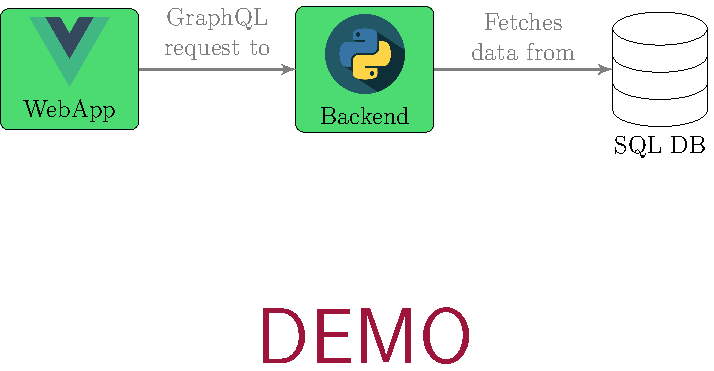
\includegraphics[width=.95\textwidth]{img/thesis_main-figure3.pdf}
    \end{figure}
  \end{center}
\end{frame}

%%%%%%%%%%%%%%%%%%%%%%%%%%%%%%%%%%%%%%%%%%%%%%%%%%%%%%%%%%%%%%%%%%%%%%%%%%%%%%%%
% NOTES:
% PaaS
%%%%%%%%%%%%%%%%%%%%%%%%%%%%%%%%%%%%%%%%%%%%%%%%%%%%%%%%%%%%%%%%%%%%%%%%%%%%%%%%
\subsection{Prototype}
\begin{frame}{}
  \vspace{-0.2cm}
  \begin{center}
    \large IoT-Management System by Symbic
  \end{center}
  \vspace{-0.2cm}
  \begin{figure}
    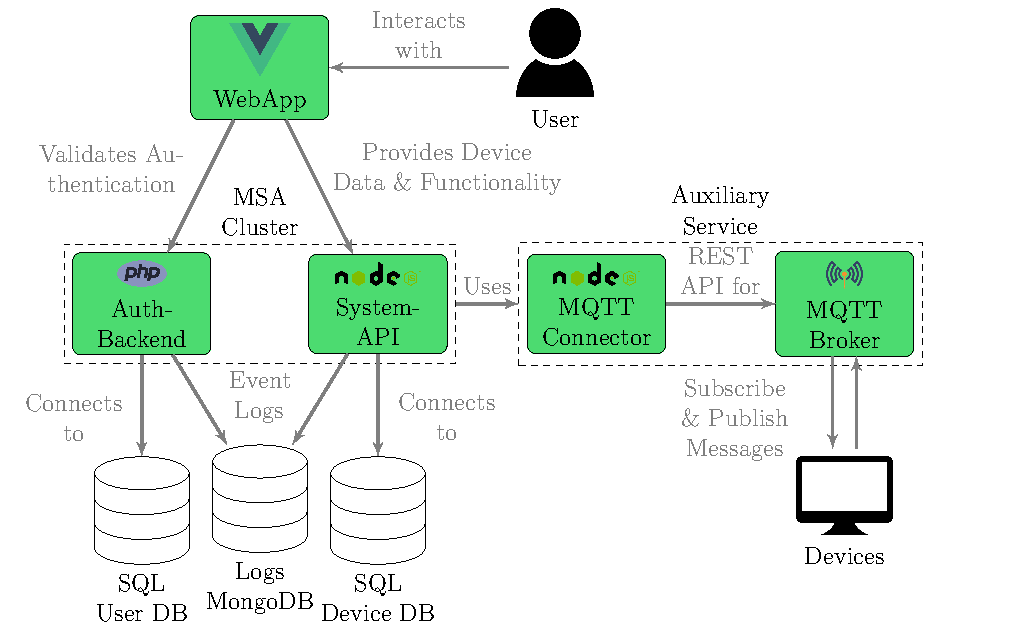
\includegraphics[width=\textwidth]{img/thesis_main-figure1.pdf}
  \end{figure}
\end{frame}

%%%%%%%%%%%%%%%%%%%%%%%%%%%%%%%%%%%%%%%%%%%%%%%%%%%%%%%%%%%%%%%%%%%%%%%%%%%%%%%%
% NOTES:
% PaaS
%%%%%%%%%%%%%%%%%%%%%%%%%%%%%%%%%%%%%%%%%%%%%%%%%%%%%%%%%%%%%%%%%%%%%%%%%%%%%%%%
\begin{frame}[fragile]{Docker-Compose}
  \begin{lstlisting}[language=docker-compose-2,basicstyle=\scriptsize,caption={Exemplary docker-compose.yml file},breaklines=true,label={code::compose_example}]
services:
  app:
    image: my-dev-image
    entrypoint: start.sh
      - DB_HOST=db
      - DB_PW=yes
      - DB_USER=root
    ports:
      - 8080:8080
    volumes:
      ./app-src:/workspace
  db:
    image: mysql
    environment:
      - MYSQL_ROOT_PASSWORD=yes
    ports:
      - 3306:3306
    \end{lstlisting}
\end{frame}




%%%%%%%%%%%%%%%%%%%%%%%%%%%%%%%%%%%%%%%%%%%%%%%%%%%%%%%%%%%%%%%%%%%%%%%%%%%%%%%%
% NOTES:
% PaaS
%%%%%%%%%%%%%%%%%%%%%%%%%%%%%%%%%%%%%%%%%%%%%%%%%%%%%%%%%%%%%%%%%%%%%%%%%%%%%%%%
\section{Applicability \& Evaluation}
\subsection{Performance Analyzes}
\begin{frame}{}
  \vspace{-.5cm}
  \begin{center}
    \Large Found properties
  \end{center}
  \begin{columns}
    \begin{column}{0.5\textwidth}
      \begin{itemize}
        \setlength\itemsep{0.6em}
        \item Faster initial setup
        \item Homogeneous environments across all developers
        \item Larger selection of software
      \end{itemize}
    \end{column}
    \begin{column}{0.5\textwidth}
      \begin{itemize}
        \setlength\itemsep{0.6em}
        \item More similar to the production environment
        \item Isolated environment to other programs
        \item More error resistant and faster error recovery
      \end{itemize}
    \end{column}
  \end{columns}

  \vspace{.5cm}
  {\color{uos-red-full}\rule{\textwidth}{1.5pt}}

  \ifx\status\final{}
    \pause{}
  \fi


  \begin{columns}
    \begin{column}{0.5\textwidth}
      \begin{itemize}
        \setlength\itemsep{0.6em}
        \item Container knowledge and infrastructure maintenance required
      \end{itemize}
    \end{column}
    \begin{column}{0.5\textwidth}
      \begin{itemize}
        \setlength\itemsep{0.6em}
        \item Noticeable performance overhead on Windows
      \end{itemize}
    \end{column}
  \end{columns}
\end{frame}


%%%%%%%%%%%%%%%%%%%%%%%%%%%%%%%%%%%%%%%%%%%%%%%%%%%%%%%%%%%%%%%%%%%%%%%%%%%%%%%%
% NOTES:
% PaaS
%%%%%%%%%%%%%%%%%%%%%%%%%%%%%%%%%%%%%%%%%%%%%%%%%%%%%%%%%%%%%%%%%%%%%%%%%%%%%%%%
\subsection{Comparison to Alternatives}
\begin{frame}
  \vspace{-.7cm}
  \begin{center}
    \Large Comparison to alternative
  \end{center}
  \vspace{-0.2cm}
  \begin{columns}[totalwidth=\textwidth]
    \begin{column}{0.5\textwidth}
      \begin{center}
        {\large\color{uos-red-full}Codesandbox.io \& Stackblitz}
      \end{center}
      \begin{itemize}
        \setlength\itemsep{0.6em}
        \item Development in a Browser with a PWA
        \item Limited programming language support
        \item Device independent with zero configuration
        \item Limited network capabilities
      \end{itemize}
    \end{column}

    \ifx\status\final{}
      \pause{}
    \fi


    \begin{column}{0.5\textwidth}
      \begin{center}
        {\large\color{uos-red-full}Codespaces \& Gitpod}
      \end{center}
      \begin{itemize}
        \setlength\itemsep{0.6em}
        \item Development in a Browser or VSCode
        \item Supports any programming language
        \item Depends on external servers
        \item Full TCP/UDP network support
      \end{itemize}
    \end{column}
  \end{columns}
\end{frame}


\subsection{Outlook}
\begin{frame}{Outlook}
  \begin{itemize}
    \large
    \setlength\itemsep{0.6em}
    \item Particularly easy to get started with - Suitable for teaching purposes and open source projects
    \item Allows programming independently of the used device
    \item Computing capacity can be flexibly adjusted
    \item Shared applications can be accessed across the team
  \end{itemize}
\end{frame}


\appendix
\begin{frame}[allowframebreaks]{References}
  \small
  \setbeamertemplate{bibliography item}[book]
  \bibliography{bib/mybib}{}
  \bibliographystyle{IEEEtranSA}
\end{frame}

\begin{frame}{Questions?}
  \begin{center}
    Thank you for your attention!

    Any questions?
  \end{center}
\end{frame}

\begin{frame}{}
  \begin{table}[]
    \scalebox{0.7}{
      \begin{tabular}{@{}lp{.18\textwidth}p{.12\textwidth}p{.12\textwidth}p{.24\textwidth}p{.18\textwidth}p{.14\textwidth}@{}}
        \toprule
                   & Orchest-ration    & Lang-uages & Server/\newline Self Hosted & Network Support & Package\newline Support        & Pricing               \\ \toprule
        Codesand                                                                                                                                             \\box.io & -                                      & NodeJS           & \checkmark/-                     & HTTP - accessible from the web             & restricted for native packages & Free, 30\$, 56\$      \\
        Stackblitz & -                & NodeJS     & -/\checkmark                      & Only WebSockets & no support for native packages & Free, 9\$, 39\$       \\
        Gitpod     & within containers & any        & \checkmark/\checkmark                     & Full TCP/UDP    & any                            & Free, 9\$, 25\$, 39\$ \\
        Code                                                                                                                                                 \\Spaces     & within containers                     & any              & \checkmark/\checkmark                    & Full TCP/UDP                               & any                            & Free, 4\$, 21\$       \\
        Dev                                                                                                                                                  \\Container   & within containers*   & any              & \checkmark/\checkmark                    & Full TCP/UDP                               & any                            & Free, 5*\$, 7*\$, 21*\$               \\
      \end{tabular}
    }
    \caption{Comparison of Different Development Solutions}\label{tab::env_compare}
  \end{table}
\end{frame}


\begin{frame}[fragile]{Dockerfile}
  \begin{lstlisting}[language=docker, frame=single, basicstyle=\footnotesize, caption={NodeJS DevContainer Dockerfile},label=code::docker_dev_node]
# Node.js version: 16-bullseye, 14-bullseye, 12-bullseye
ARG VARIANT=16-bullseye
FROM node:${VARIANT}

# Install needed packages, yarn, nvm and other tools
COPY install-scripts/*.sh /tmp/install-scripts/
RUN apt update && bash /tmp/install-scripts/install.sh \
  && apt-get -y install python3 make vim emacs git ssh \
  && npm install -g eslint
      \end{lstlisting}
\end{frame}


\begin{frame}{}
  \vspace{-0.5cm}
  \begin{center}
    \Large Testing
  \end{center}

  \vspace{-0.5cm}
  \begin{figure}
    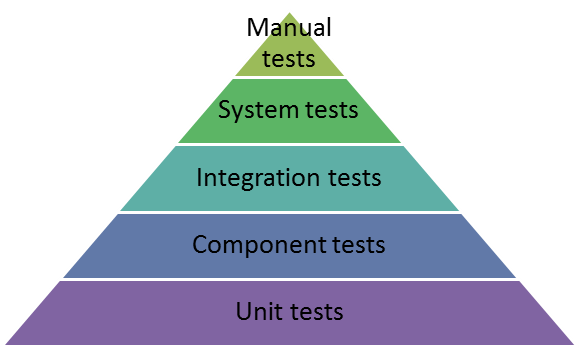
\includegraphics[width=0.58\textwidth]{img/tests-pyramid.png}
    \caption{\footnotesize The Test-Pyramid - \textcolor{uos-grey-full}{Source: {\cite{microtest}}}}
  \end{figure}
  \vspace{-0.2cm}

  \ifx\status\final{}
    \pause{}
  \fi


  \begin{block}{}
    \begin{itemize}
      \small
      \setlength\itemsep{0em}
      \item Increased testing effort in a microservice architecture
      \item Late error detection \(\Rightarrow \) higher repair costs and time
    \end{itemize}
  \end{block}
\end{frame}


\end{document}
